\documentclass[12pt]{article}
\usepackage{graphicx}
\usepackage{hyperref}
\hypersetup{
    colorlinks,
    citecolor=black,
    filecolor=black,
    linkcolor=black,
    urlcolor=black
}
\begin{document}
\tableofcontents
\section{Application layer}
\subsection{Client-server model}
In un client server model i nodi sono omogenei e il servizio è offerto da un server sempre attivo che comunica con tutti i client. 
I clients non comunicano direttamente tra loro ma c'è un server con in indirizzo IP fissato noto a tutti, così che i clients possono sempre contattarlo per ottenere il servizio. 
Spesso per gestire numerosi client vengono utilizzati più server anche se per il client è come se ci fosse un solo server.
Un applicazione web è un tipico esempio di client server model.

\subsection{P2P Peer-to-peer model}
In un P2P model i nodi sono idealmente omogenei e l'applicazione sfrutta la comunicazione tra coppie di host.
Applicazioni P2P vengono utilizzate in caso di traffico molto elevato.
Applicazioni puramente P2P sono rare, spesso si utilizza un modello ibrido tra client server e P2P. 
Un esempio è Skype che utilizza un server per la registrazione e per la ricerca di utenti, ma la comunicazione avviene direttamente tra i client.
Architetture P2P sono scalabili, distribuite e più economiche, ma sono più complesse da gestire e non sono sempre efficienti.

\subsection{Comunicazione tra Processi}
In un applicazione di rete la comunicazione avviene tra processi, ovvero tra programmi che girano su host diversi. 
Tra due processi comunicanti tipicamente che un processo client ed un processo server.
In un applicazione P2P i processo potrebbero cambiare ruolo.
Un socket è un interfaccia software che permette al processo di inviare e ricevere messaggi attraverso la rete.
Considerando lo stack TCP/IP, un socket è un interfaccia tra il livello applicazione ed il livello di trasporto.
I socket vengono utilizzati come API Application Programming Interface tra l'applicazione e la rete.
Lo sviluppatore può controllare tutto al livello applicazione ma molto poco allivello di trasporto.
L'unico controllo che ha è la scelta del protocollo di trasporto, TCP o UDP e forse la possibilità di impostare qualche parametro come la grandezza massima del buffer e del segment.
Nella rete un host viene identificato da un indirizzo IP, mentre un processo viene identificato da un numero di porta.
Alcune porte per convenzione sono riservate a determinati servizi, ad esempio la porta 80 è riservata al servizio web e la porta 25 al servizio di posta elettronica.
\subsection{Protocolli applicativi}
I protocolli del livello applicazione definiscono come i processi comunicano tra loro, ovvero il formato dei messaggi scambiati e le azioni da intraprendere quando si riceve un messaggio. 
In particolare devono definiti:
\begin{itemize}
    \item il tipo di messaggio scambiato
    \item la sintassi dei campi del messaggio
    \item la semantica dei campi del messaggio
    \item le regole per determinare quando e come un processo invia e riceve messaggi
\end{itemize}
Ci sono numerosi protocolli applicativi, alcuni dei quali sono:
\begin{itemize}
    \item HTTP/HTTPS HyperText Transfer Protocol / Secure
    \item FTP/FTPS File Transfer Protocol / Secure
    \item SMTP/SMTPS Simple Mail Transfer Protocol / Secure
    \item DNS Domain Name System
    \item DHCP Dynamic Host Configuration Protocol
    \item Telnet/SSH Telephony Network / Secure Shell
    \item SNMP Simple Network Management Protocol
\end{itemize}
\subsubsection{FTP}
FTP è uno dei protocolli più vecchio è permette il trasferimento di file tra host attraverso la rete.
Nella versione originale FTP è un protocollo non sicuro, ovvero non cripta i dati scambiati.
Mentre la versione sicura FTPS utilizza SSL/TLS per criptare i dati.
Entrambe le versioni hanno due componenti principali:
\begin{itemize}
    \item il protocollo che specifica i comandi (show, get, put, delete, etc.)
    \item un applicazione software che implementi il protocollo (client-side e server-side)
\end{itemize}
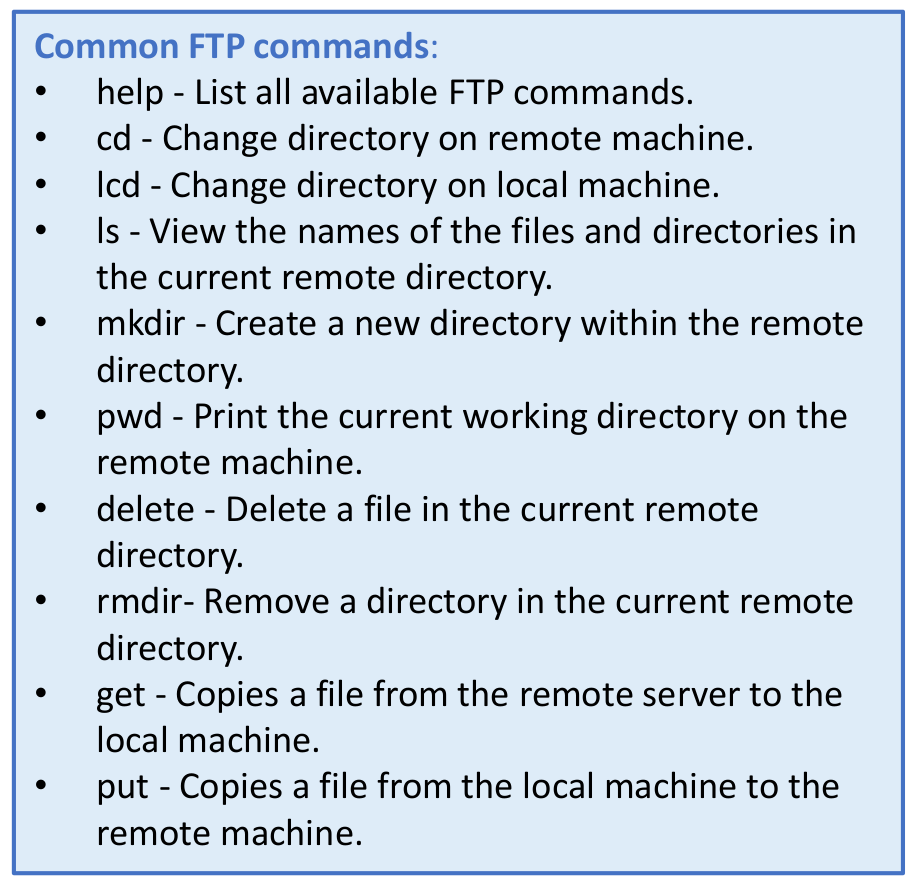
\includegraphics[scale=.3]{img/ftp-commands.png}

\subsubsection{SSH}
Telnet Telephony Network è un protocollo che permette di accedere ad un host remoto e di controllarlo come se si fosse fisicamente davanti ad esso.
Il problema è che Telnet è un protocollo non sicuro, ovvero non cripta i dati scambiati.
Per questo motivo è stato creato SSH Secure Shell che è un protocollo sicuro che utilizza SSL/TLS per criptare i dati.
Entrambe le versioni hanno due componenti principali:
\begin{itemize}
    \item il protocollo che specifica come i messaggi sono strutturati e come vengono scambiati
    \item un applicazione software che implementi il protocollo (client-side e server-side)
\end{itemize}

\subsubsection{HTTP}
Il World Wide Web WWW è un servizio che permette di accedere a documenti ipertestuali attraverso la rete.
Per accedere al WWW si utilizza il protocollo HTTP HyperText Transfer Protocol.
La comunicazione HTTP avviene tra un client ed un server.
Il client è un programma che invia richieste HTTP ad un server.
Il server è un programma che riceve le richieste HTTP ed invia una risposta HTTP.
Il protocollo HTTP definisce come i messaggi sono strutturati e come vengono scambiati.
HTTP è un protocollo non sicuro, ovvero non cripta i dati scambiati.
Per questo motivo è stato creato HTTPS che è un protocollo sicuro che utilizza SSL/TLS per criptare i dati.
Le informazioni nel web sono chiamate risorse e sono identificate da un URL Uniform Resource Locator, ovvero una stringa composta come segue:
\begin{verbatim}
[protocol]://[usrinfo@][host][:port][/path][?query][#fragment]
\end{verbatim}
\begin{itemize}
    \item protocol: protocollo di trasporto utilizzato (HTTP, HTTPS, FTP, etc.)
    \item usrinfo: nome utente e password per l'autenticazione (non più utilizzato per motivi di sicurezza)
    \item host: nome o indirizzo IP del server
    \item port: numero di porta utilizzato (spesso omesso perché dedotto dal protocollo)
    \item path: percorso della risorsa sul server
    \item query: preceduto da ?, specifica possibili richieste
    \item fragment: preceduto da \#, specifica un elemento della risorsa
\end{itemize}
Una pagina web contenete un HTML file e 5 immagini JPEG ha 6 oggetti diversi.
Il browser invia una richiesta HTTP per ogni oggetto.
Il server invia una risposta HTTP per ogni oggetto.
Il browser assembla i pezzi ricevuti e mostra la pagina web.
HTTP usa TCP come protocollo di trasporto.
Il client apre una connessione TCP con il server. Una volta che la connessione è stabilita il processo browser e quello server accedono a TCP attraverso un socket.
Il client invia una richiesta HTTP al server attraverso il socket e riceve una risposta HTTP dal server attraverso lo stesso socket. Allo stesso modo il server riceve la richiesta HTTP dal client attraverso il socket e invia la risposta HTTP attraverso lo stesso socket.
Uno dei motivi per cui HTTP usa TCP come protocollo di trasporto è che HTTP è un protocollo affidabile, ovvero garantisce che i dati inviati dal client al server arrivino correttamente e nello stesso ordine in cui sono stati inviati.
Le applicazioni HTTP delegando a TCP il compito di garantire l'affidabilità possono essere più semplici.
Per una applicazione HTTP essere semplice è molto importante perché gli permette di essere più veloce e più robusta gestendo numerose richiesta al secondo.
Le applicazioni HTTP sono generalmente stateless, ovvero non mantengono informazioni sulle richieste precedenti. Non tutte le applicazioni sono stateless, alcune applicazioni sono stateful, ovvero mantengono informazioni sulle richieste precedenti.
Il modo in cui la pagina web viene mostrata al client dipende dal tipo di browser utilizzato. Il protocollo HTTP definisce soltanto come i messaggi sono strutturati e come vengono scambiati, non definisce come la pagina web deve essere mostrata al client.
In molte applicazioni web il client ed il server comunicano per un periodo esteso di tempo, inviando e ricevendo messaggi in sequenza.
Quando utilizziamo una connessione TCP possiamo avere due tipi di connessione: persistente e non persistente.
Una connessione persistente è una connessione TCP che viene riutilizzata per più di una richiesta HTTP.
Una connessione non persistente è una connessione TCP che viene utilizzata per una sola richiesta HTTP.
Siccome la connessione non persiste tra una richiesta e l'altra c'è bisogno di tante connessione TCP per scaricare l'intera pagina web.
La connessione avviene come segue:
\begin{enumerate}
    \item Il processo client HTTP inizia una connessione TCP con il server \texttt{www.someSchool.edu} sulla porta numero 80 (default per HTTP), avremo quindi due socket: uno nel client e uno nel server.a
    \item Il client HTTP invia un messaggio di richiesta HTTP al server tramite il suo socket, includendo il nome del percorso \texttt{/someDepartment/home.index}.
    \item Il processo server HTTP riceve il messaggio di richiesta tramite il suo socket, recupera l'oggetto \texttt{/someDepartment/home.index} (da RAM o disco), incapsula l'oggetto in un messaggio di risposta HTTP e invia indietro il messaggio di risposta al client tramite il suo socket.
    \item Il processo server HTTP dice a TCP di chiudere la connessione TCP; il TCP (più tardi) terminerà la connessione una volta che è sicuro che il client ha ricevuto il messaggio di risposta intatto (affidabilità).
    \item Il client HTTP riceve il messaggio di risposta. La connessione TCP termina. Il messaggio indica che l'oggetto incapsulato è un file HTML. Il client estrae il file dal messaggio di risposta, esamina il file HTML e trova riferimenti ai 10 oggetti JPEG.
    \item I primi quattro passaggi vengono quindi ripetuti per ciascuno degli oggetti JPEG referenziati.
\end{enumerate}
Le diverse connessione possono essere aperte in sequenza o in parallelo.
Nonostante il parallelismo, creare tante connessioni TCP è molto costoso in termini di tempo e risorse.
È difficile stimare precisamente i tempi di una richiesta HTTP.
Una possibile stima può essere fatta in termini di RTTs round-trip times, ovvero il tempo che impiega un pacchetto per andare dal client al server e ritornare indietro.
Le connessioni TCP sono garantite (connection-oriented) grazie al three-way handshake.
Il three-way handshake è una procedura che permette di stabilire una connessione TCP tra due host attraverso 3 passaggi:
\begin{enumerate}
    \item il client invia un piccolo segmento TCP al server per segnalare la richiesta di connessione.
    \item il server risponde con un piccolo segmento TCP per segnalare l'accettazione della richiesta di connessione.
    \item il client invia un piccolo segmento TCP per confermare l'accettazione della richiesta di connessione.
\end{enumerate}
Per terminare la procedura servono 2 RTTs. La stessa procedura viene utilizzata per terminare la connessione.
Se la connessione è persistente, il client può inviare più richieste HTTP attraverso la stessa connessione TCP.
In questo modo si riduce il numero di RTTs necessari per scaricare la pagina web.
Se la connessione è non persistente, il client deve aprire una nuova connessione TCP per ogni richiesta HTTP e quindi il numero di RTTs necessari per scaricare la pagina web aumenta.
Quando utilizziamo una connessione persistente possiamo inviare le richieste in pipeline, ovvero possiamo inviare una nuova richiesta HTTP prima di aver ricevuto la risposta alla richiesta precedente.
Nel protocollo HTTP abbiamo due formati diversi per i messaggi di richiesta e di risposta.
Il formato dei messaggi di richiesta HTTP è il seguente:
\begin{verbatim}
    <method> <URL> <version>
    <headers>
    <body>
\end{verbatim}
\begin{itemize}
    \item method: tipo di richiesta (GET, POST, HEAD, PUT, DELETE, etc.)
    \item URL: Uniform Resource Locator
    \item version: versione del protocollo HTTP (HTTP/1.1)
    \item headers: parametri della richiesta (es persistent o non persistent connection)
    \item body: dipende dal tipo di richiesta (per GET è vuoto), contiene i dati utilizzati dal metodo.
\end{itemize}
Il metodo GET è il più utilizzato e permette di richiedere una risorsa.
\begin{verbatim}
GET /somedir/page.html HTTP/1.1
Host: www.someschool.edu
Connection: close
User-agent: Mozilla/5.0
Accept-language: fr
\end{verbatim}
Il metodo POST permette di inviare dati al server.
Il metodo HEAD è simile a GET ma il server risponde soltanto con l'header della risposta. Viene utilizzato per testare l'esistenza di una risorsa.
Il metodo PUT permette di caricare una pagina web sul server.
Il metodo DELETE permette di cancellare una pagina web dal server.
Il formato dei messaggi di risposta HTTP è il seguente:
\begin{verbatim}
    <version> <status-code> <reason-phrase>
    <headers>
    <body>
\end{verbatim}
\begin{itemize}
    \item version: versione del protocollo HTTP
    \item status: codice di stato (200 OK, 301 Moved Permanently, 400 Bad Request, 404 Not Found, 505 HTTP Version Not Supported, etc.)
    \item reason-phrase: descrizione del codice di stato
\end{itemize}
Status codes sono divisi in classi:
\begin{itemize}
    \item 100-199: informational (richiesta ricevuta, processo in corso, etc.)
    \item 200-299: successful
    \item 300-399: redirection (ci sono azioni da intraprendere da parte dell'utente per completare la richiesta)
    \item 400-499: client error (richiesta non valida)
    \item 500-599: server error (server non riesce a soddisfare la richiesta)
\end{itemize}
Alcuni esempi di status codes sono:
\begin{itemize}
    \item 200 OK: richiesta soddisfatta
    \item 301 Moved Permanently: la risorsa è stata spostata in un'altra locazione
    \item 400 Bad Request: richiesta non valida
    \item 404 Not Found: la risorsa non è stata trovata
    \item 505 HTTP Version Not Supported: la versione del protocollo HTTP non è supportata
\end{itemize}
Esempio di risposta HTTP:
\begin{verbatim}
HTTP/1.1 200 OK
Connection: close
Date: Tue, 18 Aug 2015 15:44:04 GMT
Server: Apache/2.2.3 (CentOS)
Last-Modified: Tue, 18 Aug 2015 15:11:03 GMT
Content-Length: 6821
Content-Type: text/html
(data data data data data ...)
\end{verbatim}
\subsubsection{Cookies}
I server HTTP sono stateless, ovvero non mantengono informazioni sulle richieste precedenti.
I cookies sono un meccanismo che permette ai server HTTP di mantenere informazioni sulle richieste precedenti.
Un cookie è un token digitale che il server una ser identificare un utente.
Un cookie viene creato dal server ed inviato al client.
La tecnologia dei cookie utilizza 4 componenti principali:
\begin{itemize}
    \item un set-cookie header nel messaggio di risposta HTTP
    \item un cookie header nel messaggio di richiesta HTTP
    \item un file di cookie mantenuto dal browser
    \item un back-end database sul server
\end{itemize}
\subsubsection{Proxy}
Una Web cache anche chiamato proxy server è un server che mantiene copie di pagine web recentemente richieste.
Quando un client richiede una pagina web, il proxy server controlla se ha una copia della pagina web.
Se il proxy server ha una copia della pagina web, invia la copia al client.
Se il proxy server non ha una copia della pagina web, il proxy server richiede la pagina web al server originale, invia la copia al client e mantiene una copia per le richieste future.
Il proxy server può essere utilizzato per:
\begin{itemize}
    \item ridurre il tempo di risposta per le richieste HTTP
    \item ridurre il traffico sulla rete
    \item ridurre il traffico sul server originale
    \item filtrare i contenuti
    \item tracciare le attività degli utenti 
    \item mascherare i server originale
\end{itemize}
La copia della pagina web mantenuta dal proxy server potrebbe essere obsoleta.
Per questo motivo il proxy server deve controllare se la copia è ancora valida.
Per controllare se la copia è ancora valida il proxy server invia una richiesta HTTP conditional GET al server originale con un if-modified-since nell'header.
Se la copia è ancora valida il server originale risponde con un not modified status code.
Se la copia non è più valida il server originale risponde con un ok status code e invia la nuova copia al proxy server.
Il caching può essere fatto anche dal client nel browser.

\subsubsection{SMTP}
Simple Mail Transfer Protocol è un protocollo che permette di inviare e ricevere email.
Ci sono due tipi di agenti:
\begin{itemize}
    \item User Agent che permette di comporre, leggere e inviare email (es Outlook, Thunderbird, etc.)
    \item Mail Server che permette di ricevere, inoltrare e consegnare email
\end{itemize}
Il protocollo SMTP è un protocollo client-server che utilizza la connessione TCP sulla porta 25.
Per prima cosa il client crea una connessione TCP con il server sulla porta 25.
Il server ed il client eseguono la procedura three-way handshake per stabilire la connessione TCP.
Per ottenere le mail dal server abbiamo bisogno si un protocollo di accesso alle email.
I protocolli di accesso alle email sono:
\begin{itemize}
    \item POP3 Post Office Protocol version 3
    \item IMAP Internet Mail Access Protocol
    \item HTTP
\end{itemize}
POP3 è un protocollo client-server che utilizza la connessione TCP sulla porta 110.
con POP3 le email vengono scaricate dal server e salvate sul client.
IMAP è un protocollo client-server che utilizza la connessione TCP sulla porta 143.
Con IMAP le email rimangono sul server e vengono scaricate dal client quando necessario.
Inoltre IMAP permette di organizzare le email in cartelle, di fare ricerche ecc.
HTTP è un protocollo client-server che utilizza la connessione TCP sulla porta 80.

\subsubsection{DNS}
Il Domain Name System è un protocollo di applicazione che permette di mappare un nome di dominio ad un indirizzo IP.
Il DNS è un protocollo client-server che utilizza la connessione UDP sulla porta 53.
Ad esempio se il browser vuole accedere a \texttt{www.someSchool.edu/index.html} invia una richiesta DNS al server DNS.
Il browser estrae il nome dell'host \texttt{www.someSchool.edu} dal URL e lo utilizza  nella come parametro nella funzione gethosybyname() in C/C++ per ottenere l'indirizzo IP dell'host. All'invocazione della funzione avvengono i seguenti passaggi:
\begin{enumerate}
    \item Il DNS Client manda una query UDP al server DNS sulla porta 53 contenente il nome dell'host.
    \item Il DNS Client riceve una risposta UDP dal server DNS contenente l'indirizzo IP dell'host.
\end{enumerate}
Una volta che il browser ha l'indirizzo IP dell'host può inviare una richiesta HTTP al server HTTP alla porta 80.
Il DNS è un protocollo distribuito, ovvero non c'è un server DNS centrale.
Il DNS è un protocollo gerarchico, ovvero i server DNS sono organizzati in una gerarchia.
Ci sono 3 tipi di server DNS:
\begin{itemize}
    \item root DNS server
    \item top-level domain DNS server
    \item authoritative DNS server
\end{itemize}
Quando un client DNS vuole un indirizzo IP invia una richiesta al server DNS root.
Il server DNS root risponde con l'indirizzo IP del server DNS top-level domain appropriato (es .edu, .com, .it, etc.).
Il client DNS invia una richiesta al server DNS top-level domain.
Il server DNS top-level domain risponde con l'indirizzo IP del server DNS authoritative appropriato (es someSchool.edu).
Il client DNS invia una richiesta al server DNS authoritative.
Il server DNS authoritative risponde con l'indirizzo IP dell'host.
Esiste un altro tipo di server DNS chiamato local DNS server.
Tipicamente il local DNS server è gestito dal provider di servizi internet ISP.
Il local DNS server mantiene una cache delle richieste DNS recenti come un proxy server.
I DNS server offrono anche un servizio di aliasing, ovvero permettono di associare un nome di dominio ad un altro nome di dominio così da avere un indirizzo ip associato a più nomi di dominio.
I DNS server dato un indirizzo IP permettono di ottenere il nome o nomi di dominio associati.
Un DNS server può essere utilizzato per applicare la load distribution, ovvero per distribuire il carico tra più server.
Siti molto grandi come Google, Facebook, Amazon, etc. hanno molti server.
Per distribuire il carico tra i server questi siti utilizzano un DNS server che mappa un nome di dominio ad un insieme di indirizzi IP.
Quando un client invia una richiesta DNS al server DNS, il server DNS risponde con un indirizzo IP scelto tra quelli disponibili.
In questo modo il carico viene distribuito tra i server.

\subsubsection{Torrent}
Uno degli utilizzi di un applicazione P2P è la condivisione di file.
Un protocollo P2P per la condivisione di file è BitTorrent.
Un Torrent è una collezione di peers che partecipano alla condivisione di un file.
Peers in un torrent scaricano chunks di dimensione fissa da altri peers e li inviano ad altri peers.
Quando un peer entra in un torrent non ha nessun chunk, quindi inizia scaricando un chunk da un peer che ha quel chunk.
Una volta che ha scaricato un chunk lo invia ad altri peer che non hanno quel chunk.
Un peer appena entrato si registra presso un tracker che mantiene una lista di peers che partecipano al torrent.
Il tracker risponde al peer con una lista di peers da cui ottenere chunks.
Il peer si connette ai peers della lista e inizia a scaricare chunks.
Ogni peer puo uscire e rientrare nel torrent in qualsiasi momento.
Un peer si collega agli altri peer attraverso un socket TCP.
Un peer può avere più connessioni TCP contemporaneamente.
Per la scelta dei chunks da scaricare un peer utilizza un algoritmo chiamato rarest first.
L'algoritmo rarest first sceglie i chunks che sono posseduti da meno peers.
In questo modo si cerca di massimizzare la disponibilità dei chunks.
Per la scelta dei chunks da caricare si possono usare due algoritmi:
Trading: il peer da priorità hai 4 vicini che stanno caricando più chunks, con aggiornamenti ogni 10 secondi.
Random selection: ogni 30 secondi il peer sceglie 4 vicini a caso.


\end{document}